%! TeX program = lualatex
\documentclass[notes, 10pt, aspectratio=169]{beamer}
%\documentclass[10pt, aspectratio=169]{beamer}

\usepackage{booktabs}
\usepackage[style=verbose,backend=biber]{biblatex}
\addbibresource{../report/main.bib}

% notes
%\usepackage{pgfpages}
%\setbeamertemplate{note page}[plain]
%\setbeameroption{show notes on second screen=right}
\graphicspath{{../report/graphics/}}

\usetheme[style=fwn]{leidenuniv}
\useinnertheme{circles}
\useoutertheme[subsection=false]{miniframes}
\beamertemplatenavigationsymbolsempty

% uncomment next line to let framesubtitle have palette primary color
%\setbeamercolor{framesubtitle}{use={palette primary},fg=palette primary.bg}

% uncomment next line to remove navigation symbols from the pdf
%\setbeamertemplate{navigation symbols}{}

\title{CRET: Cross-Modal Retrieval Transformer for Efficient Text-Video Retrieval}
\subtitle{Authors: Kaixiang Ji, Jiajia Liu, Weixiang Kong, Liheng Zhong, Jian Wang, Jingdong Chen, Wei Chu}
\author{Siwen Tu and Shupei Li}
\institute[LIACS]{Leiden Institute of Advanced Computer Science}
\date{April 11, 2023}


\begin{document}

\begin{frame}[plain]
	\titlepage
\end{frame}

\begin{frame}
	\tableofcontents
\end{frame}

\section{Motivation}
\begin{frame}
    \frametitle{Motivation}
    \begin{itemize}
        \item Unimodal information retrieval task.
            \vspace{0.1cm}
            \begin{center}
                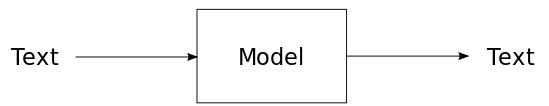
\includegraphics[width=7cm]{single-modality.png}
            \end{center}
            \vspace{0.1cm}
        \item Multimodal information retrieval task, e.g. text-to-video retrieval.
            \vspace{0.1cm}
            \begin{center}
                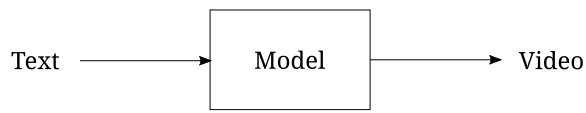
\includegraphics[width=7cm]{multimodality.png}
            \end{center}
    \end{itemize}
\end{frame}

\section{Methodololgy}
\begin{frame}
    \frametitle{EDB method versus MDB method}
    \begin{center}
        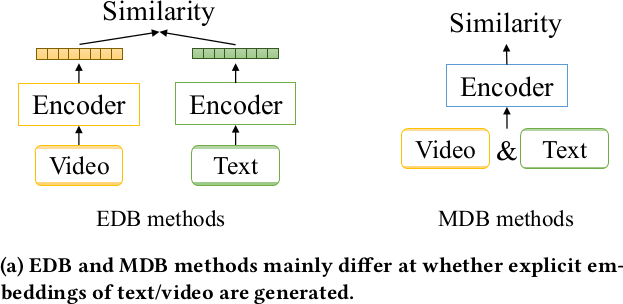
\includegraphics[width=8cm]{edb-mdb.png}
    \end{center}
    \begin{itemize}
        \item EDB method: Inferior performance due to the lack of feature alignment.
        \item MDB method: Low efficiency due to the exhaustive scan over the entire database.
    \end{itemize}
\end{frame}

\begin{frame}
    \frametitle{Overview of the CRET model}
    \begin{center}
        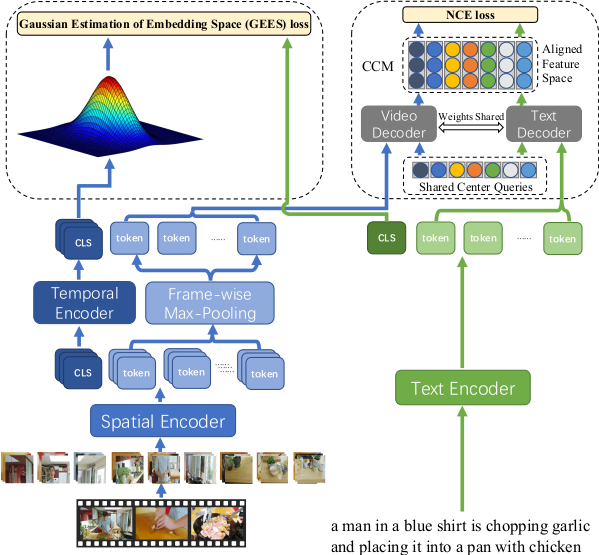
\includegraphics[width=7cm]{model.png}
    \end{center}
\end{frame}

\begin{frame}
    \frametitle{Two main contributions: CCM \& GEES}
    \textbf{Cross-modal correspondence modeling (CCM)}
    \begin{itemize}
        \item Utilize transformer decoders to align the features from text and video modalities. 
        \item Use queries as common centers of features from both modalities.
        \item Parameters are shared between decoders of two modalities.
    \end{itemize}
    \textbf{Gaussian estimation of embedding space (GEES)}
    \begin{align*}
        \mathbf{Z}_{c,j} = \text{softmax}\left( \frac{(Q_cW_j^Q)(EW_j^K)^T}{\sqrt{d_k}} \right) (EW_j^V)
    \end{align*}
    \begin{enumerate}
        \item Calculate the distance between token features and the query center. Regard the distance as the weight of corresponding features.
        \item Concatenate and project the aligned features.
        \item Calculate the similarity score of features from text and video modalities.
    \end{enumerate}
\end{frame}

\section{Experiments}
\begin{frame}
    \frametitle{Experiments} 
    \begin{itemize}
        \item \textbf{Datasets}: MSRVTT, LSMDC, MSVD, DiDeMo.
        \item \textbf{Metrics}: R@K, MdR.
        \item \textbf{Results}:
            \begin{itemize}
                \item MSRVTT
                    \vspace{0.1cm}
                    \begin{center}
                        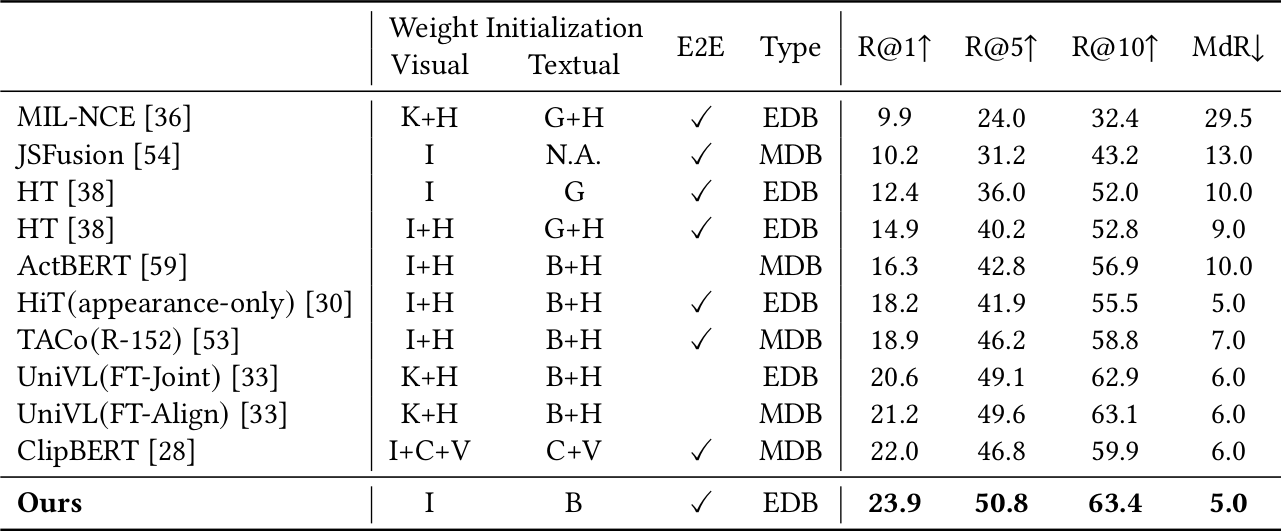
\includegraphics[width=10cm]{msrvtt.png}
                    \end{center}
            \end{itemize}
    \end{itemize}
\end{frame}

\begin{frame}
    \frametitle{Experiments}
    \begin{itemize}
        \item \textbf{Results}:
    \begin{itemize}
        \item LSMDC
            \begin{center}
                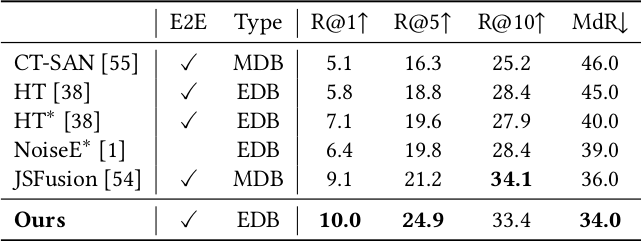
\includegraphics[width=8cm]{lsmdc.png}
            \end{center}
        \item MSVD
            \begin{center}
                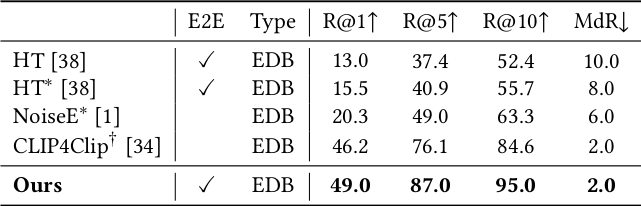
\includegraphics[width=8cm]{msvd.png}
            \end{center}
    \end{itemize}
    \end{itemize}
\end{frame}

\begin{frame}
    \frametitle{Experiments}
    \begin{itemize}
        \item \textbf{Results}:
    \begin{itemize}
        \item DiDeMo
            \begin{center}
                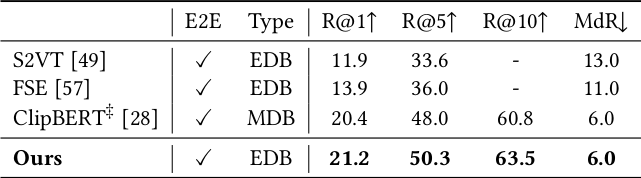
\includegraphics[width=8cm]{didemo.png}
            \end{center}
    \end{itemize}
\item \textbf{Ablation studies}.
\item \textbf{Validation of Gaussian assumption}.
    \end{itemize}
\end{frame}

\section{Critical Review}
\begin{frame}
    \frametitle{Critical review} 
    \begin{itemize}
        \item Readability and structure.
            \begin{itemize}
                \item Illustrate CRET method clearly.
                \item Satisfy requirements of the scientific paper.
            \end{itemize}
        \item Reproducibility: Source code, the availability of data sets, experimental settings.
        \item Importance.
            \begin{itemize}
                \item Theoretical contributions.
                \item Practical applications.
            \end{itemize}
        \item Summary of strong and weak points.
    \end{itemize}
\end{frame}

\section*{Appendix}
\begin{frame}
    \frametitle{Appendix: Details of GEES}
    Vanilla NCE loss:
    \begin{align*}
        \mathcal{L}_{NCE} = \frac{1}{N}\sum_{i = 1}^N \frac{1}{M}\sum_{j = 1}^M -\log \left( \frac{\exp \left( <V_{ij}^g, T_i^g> \right) }{\exp\left( <V_{ij}^g, T_i^g> \right) + \sum_{(V^{g'}, T^{g'})\in \Phi_i}\exp\left( <V^{g'}, T^{g'}> \right) } \right) 
    \end{align*}
    Multivariate Gaussian distribution assumption:
    \begin{align*}
        v_i\sim \mathcal{N}\left( \mu_i, \sigma_i \right) 
    \end{align*}
    Derive the GEES and its upper bound:
    \begin{align*}
        \mathcal{L}_{GEES} &= \frac{1}{N}\sum_{i = 1}^N E_{v_i} \left[ -\log \left(  \frac{\exp \left( <V_{ij}^g, T_i^g> \right) }{\exp\left( <V_{ij}^g, T_i^g> \right) + \sum_{(V^{g'}, T^{g'})\in \Phi_i}\exp\left( <V^{g'}, T^{g'}> \right) }  \right)  \right] \\
                           &\leq -\frac{1}{N}\sum_{i = 1}^N\log \frac{\exp\left( <T_i^g, \mu_i> + \frac{1}{2}<T_i^g, \sigma_iT_i^g> \right) }{\sum_{j=1}^N\exp\left( <T_i^g, \mu_i> + \frac{1}{2}<T_i^g, \sigma_iT_i^g> \right) } = \bar{\mathcal{L}}_{GEES}
    \end{align*}
\end{frame}

\begin{frame}
    \frametitle{Strategies of training and inference}
    Training:
    \begin{align*}
    \mathcal{L}_{CCM}&= -\frac{1}{N}\sum_{i = 1}^N-\log \left( \frac{\exp\left( <Z_i^v, Z_i^t> \right) }{\exp\left( Z_i^v, Z_i^t \right)+\sum_{(Z^{v'}, Z^{t'})\in \Psi_i}\exp\left( <Z^{v'}, Z^{t'}> \right)  } \right) \\
    \mathcal{L}_{total} &= \bar{\mathcal{L}}_{GEES} + \alpha \mathcal{L}_{CCM}
    \end{align*}
    Inference:
    \begin{align*}
        S &= S_g + \beta S_l\\
        S_l &= \cos\left( Z^v, Z^t \right) \\
        S_g &= \cos\left( \frac{1}{M}\sum_{j = 1}^M V_{ij}^g, T_i^g \right) 
    \end{align*}
\end{frame}
\end{document}
